\documentclass[10pt]{beamer}

\usepackage[utf8]{inputenc}
\usepackage{tcolorbox}
\usepackage{tikz}
\usepackage{tikz-3dplot}
\usetikzlibrary{intersections,calc,,angles,quotes,through}
\usepackage{amsmath}
\usepackage{graphicx}
\usepackage{cases}
\def \heart {\textcolor{blue}{$\heartsuit$} }
\def \C {\mathcal{C}}
\def \orthog {\underline{\perp}}
\def\arcos{\operatorname{arcos}}
\def \deg {^{\circ}}

\newcommand{\vect}[1] {
  \overrightarrow{#1}}

\tcbset{%
	basic/.style={colframe=black,
		      colback=white,
		      top= 0mm,
		      bottom = 2mm,
		      boxsep=0mm
		      }
}
\tikzset{
    invisible/.style={opacity=0},
    visible on/.style={alt={#1{}{invisible}}},
    alt/.code args={<#1>#2#3}{%
      \alt<#1>{\pgfkeysalso{#2}}{\pgfkeysalso{#3}} % \pgfkeysalso doesn't change the path
    },
  }

    
\begin{document}  
    \beamertemplatenavigationsymbolsempty
    \setlength{\abovedisplayskip}{0pt}
    \setlength{\belowdisplayskip}{0pt}
    \frame{
	  
	  \frametitle{Exercice sur le calcul de barycentre.}
	  \renewcommand{\theenumi}{\alph{enumi})}
	  Soit $ABC$ un triangle et $M$ un point quelconque du plan $ABC$. Soient
	  $M_1$ , $M_2$ et $M_3$ les points symétriques respectifs de $M$ par rapport aux
	  milieux des segments $[BC]$, $[CA]$ et $[AB]$. On note $G$ et $K$ les centre de
	  gravité respectifs des triangles $ABC$ et $M_1M_2M_3$.
	  \begin{enumerate}
	   \item Démontrer que $\vect{MK}=2\vect{MG}$.
	   \item Démontrer que les trois segments $[AM_1]$,$[BM_2]$ et $[CM_3]$ ont
		 même milieu $I$. Justifier que le point $I$ est milieu de $[GK]$.
	  \end{enumerate}

	  \vfill
	  
	  \pause
	  % hypothèses et thèse
	  \begin{tcolorbox}[basic] 
	      \begin{columns}[t]
		 
		 \column{.5\textwidth}\centering
		      
		      \underline{Hypothèses} 
		      \begin{itemize}
		      \item $G$ centre de gravité de $\Delta ABC$,
		      \item $M_1,M_2,M_3$ symétriques de $M$ p/r aux côtés du $\Delta ABC$,
		      \item $K$ centre de gravité de $\Delta M_1M_2M_3$.		     
		      \end{itemize}

		  
		  \column{.5\textwidth}\centering
		      
		      \underline{Thèse} 
		      \begin{enumerate}
		       \item $\vect{MK}=2\vect{MG}$,
		       \item Milieux de $[AM_1]$, $[BM_2]$,\\ \smallskip $[CM_3], [GK]$ confondus.
		      \end{enumerate}

		
	      \end{columns}
	  \end{tcolorbox}
	  {\small Référence : SORTAY Y.,SORTAY R.,1988. \textit{Géométrie de l'espace
	  et du plan}. Herman, 394p.}
    }

    \frame{ 
	  % résolution ex1
	  \begin{columns}[t]
		\column{.565\textwidth}\centering 
		

			\underline{Dessin}\\
				  \vspace{-3mm}
				  \begin{figure}[h]
				  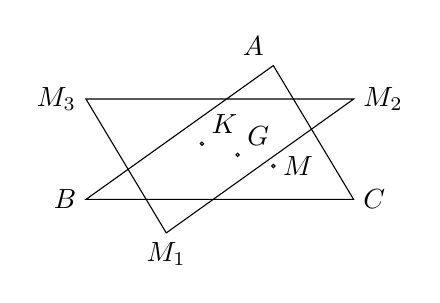
\begin{tikzpicture}[scale=0.85]
			          %projection ($(X)!(B')!(B)$)
			          %nommer chemin 'name path
			          %intersection \path [name intersections={of=d and gb,name=G}];
			          %animation  \draw[visible on=<1>] 
				  %           \draw[visible on=<{2,4}>]
				  %angle arc[radius = 6mm, start angle= 180, end angle= 225] node [below left,pos=0.3]{$\alpha$}
				  %angle \pic [draw,"$\alpha$", angle eccentricity=1.5] {angle = A'--A--B};
				  %perpendiculaire ($(A')!3cm!-90:(A)$)
				  %cercle par point \node [draw] at (A) [circle through=(B)] {};
				   
				  %TRIANGLE ABC
				  \coordinate[label= above left:$A$](A) at (0.8,2);
				  \coordinate[label=left:$B$](B) at (-2,0);
				  \coordinate[label=right:$C$](C) at (2,0);
				  \draw (A) -- (B) -- (C) -- cycle;
				  
				  %M,M_1,M_2,M_3
				  \coordinate[label=right:$M$](M) at (0.8,0.5);
				  \draw (M) circle (0.025);
				  \path (M) -- +($2*(B)!.5!(C)-2*(M)$) coordinate[label=below:$M_1$](M_1);
				  \path (M) -- +($2*(A)!.5!(C)-2*(M)$) coordinate[label=right:$M_2$](M_2);
				  \path (M) -- +($2*(A)!.5!(B)-2*(M)$) coordinate[label=left:$M_3$](M_3);
				  \draw (M_1) -- (M_2) -- (M_3) -- cycle;
				  
				  %G,K
				  \coordinate[label=above right:$G$](G) at ($.333*(A)+.333*(B)+.333*(C)$);
				  \draw (G) circle (0.025);
				  \coordinate[label=above right:$K$](K) at ($.333*(M_1)+.333*(M_2)+.333*(M_3)$);
				  \draw (K) circle (0.025);
				  \end{tikzpicture}
				  \end{figure}
				  \vspace{-4mm}
				  \begin{tcolorbox}[basic] 
				      
				    \smallskip
				    \underline{Hypothèses} 
				    \begin{enumerate}
				    \item $G$ centre de gravité de $\Delta ABC$,
				    \item $M_1,M_2,M_3$ symétriques de $M$ p/r aux côtés du $\Delta ABC$,
				    \item $K$ centre de gravité de $\Delta M_1M_2M_3$.    
				    \end{enumerate}
							      
				    \underline{Thèse}
				    \renewcommand{\theenumi}{\alph{enumi})}
				    \begin{enumerate}
				    \item $\vect{MK}=2\vect{MG}$,
				    \item Milieux de $[AM_1]$, $[BM_2]$,\\ \smallskip $[CM_3], [GK]$ confondus.
				    \end{enumerate}
				    \end{tcolorbox}
		
		
		\column{.5\textwidth}\centering
		
		\underline{Résolution}\\ \flushleft
		
		\begin{enumerate}
		 \item $\vect{MG}= \frac{1}{3}\vect{MA} + \frac{1}{3}\vect{MB} + \frac{1}{3}\vect{MC}$,\\[1em]
		 \item  $\vect{MM_1}=\ 2\ (\frac{1}{2}\vect{MB} + \frac{1}{2}\vect{MC})$, \\[0.5em]
			$\vect{MM_2}=\ 2\ (\frac{1}{2}\vect{MA} + \frac{1}{2}\vect{MC})$, \\[0.5em]
			$\vect{MM_3}=\ 2\ (\frac{1}{2}\vect{MA} + \frac{1}{2}\vect{MB})$, \\[1em]
		 \item \begin{align*}
		         \vect{MK}=\ & \frac{1}{3}\vect{MM_1} + \frac{1}{3}\vect{MM_2} + \frac{1}{3}\vect{MM_3}, \\[0.5em]
				  =\ & 2\ (\frac{1}{3}\vect{MA} + \frac{1}{3}\vect{MB} + \frac{1}{3}\vect{MC}), \\[0.5em]
				  =\ & 2\vect{MG}.
		       \end{align*}
		\end{enumerate}	
		\hfill $\qed(a)$ \\

	   \end{columns}   
    }
	
        \frame{ 
	  % résolution ex1
	  \begin{columns}[t]
		\column{.565\textwidth}\centering 
		

			\underline{Dessin}\\
				  \vspace{-3mm}
				  \begin{figure}[h]
				  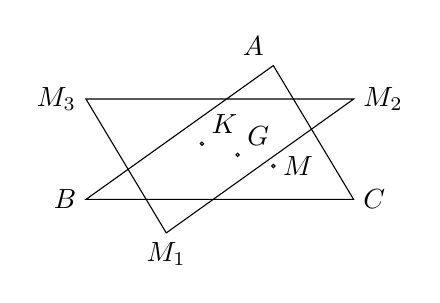
\begin{tikzpicture}[scale=0.85]
			          %projection ($(X)!(B')!(B)$)
			          %nommer chemin 'name path
			          %intersection \path [name intersections={of=d and gb,name=G}];
			          %animation  \draw[visible on=<1>] 
				  %           \draw[visible on=<{2,4}>]
				  %angle arc[radius = 6mm, start angle= 180, end angle= 225] node [below left,pos=0.3]{$\alpha$}
				  %angle \pic [draw,"$\alpha$", angle eccentricity=1.5] {angle = A'--A--B};
				  %perpendiculaire ($(A')!3cm!-90:(A)$)
				  %cercle par point \node [draw] at (A) [circle through=(B)] {};
				   
				  %TRIANGLE ABC
				  \coordinate[label= above left:$A$](A) at (0.8,2);
				  \coordinate[label=left:$B$](B) at (-2,0);
				  \coordinate[label=right:$C$](C) at (2,0);
				  \draw (A) -- (B) -- (C) -- cycle;
				  
				  %M,M_1,M_2,M_3
				  \coordinate[label=right:$M$](M) at (0.8,0.5);
				  \draw (M) circle (0.025);
				  \path (M) -- +($2*(B)!.5!(C)-2*(M)$) coordinate[label=below:$M_1$](M_1);
				  \path (M) -- +($2*(A)!.5!(C)-2*(M)$) coordinate[label=right:$M_2$](M_2);
				  \path (M) -- +($2*(A)!.5!(B)-2*(M)$) coordinate[label=left:$M_3$](M_3);
				  \draw (M_1) -- (M_2) -- (M_3) -- cycle;
				  
				  %G,K
				  \coordinate[label=above right:$G$](G) at ($.333*(A)+.333*(B)+.333*(C)$);
				  \draw (G) circle (0.025);
				  \coordinate[label=above right:$K$](K) at ($.333*(M_1)+.333*(M_2)+.333*(M_3)$);
				  \draw (K) circle (0.025);
				  \end{tikzpicture}
				  \end{figure}
				  \vspace{-4mm}
				  \begin{tcolorbox}[basic] 
				      
				    \smallskip
				    \underline{Hypothèses} 
				    \begin{enumerate}
				    \item $G$ centre de gravité de $\Delta ABC$,
				    \item $M_1,M_2,M_3$ symétriques de $M$ p/r aux côtés du $\Delta ABC$,
				    \item $K$ centre de gravité de $\Delta M_1M_2M_3$.    
				    \end{enumerate}
							      
				    \underline{Thèse}
				    \renewcommand{\theenumi}{\alph{enumi})}
				    \begin{enumerate}
				    \item $\vect{MK}=2\vect{MG}$,
				    \item Milieux de $[AM_1]$, $[BM_2]$,\\ \smallskip $[CM_3], [GK]$ confondus.
				    \end{enumerate}
				    \end{tcolorbox}
		
		
		\column{.5\textwidth}\centering
		
		\underline{Résolution}\\ \flushleft
		\begin{align*}
		 \frac{1}{2}\vect{MK} + \frac{1}{2}\vect{MG} = \ & \frac{3}{2}\vect{MG} \text{ ( \textcolor{blue}{a.} )} \\
							     = \ & \frac{1}{2}\vect{MA} + \frac{1}{2}\vect{MB} + \frac{1}{2}\vect{MC} \\[1.5em]
		 \frac{1}{2}\vect{MA} + \frac{1}{2}\vect{MM_1} = \ & \frac{1}{2}\vect{MA} + \frac{1}{2}\vect{MB} + \frac{1}{2}\vect{MC} \\[0.7em]
		 \frac{1}{2}\vect{MB} + \frac{1}{2}\vect{MM_2} = \ & \frac{1}{2}\vect{MA} + \frac{1}{2}\vect{MB} + \frac{1}{2}\vect{MC} \\[0.7em] 
		 \frac{1}{2}\vect{MC} + \frac{1}{2}\vect{MM_3} = \ & \frac{1}{2}\vect{MA} + \frac{1}{2}\vect{MB} + \frac{1}{2}\vect{MC} 
		\end{align*}
		\bigskip
		
		Milieux de $[AM_1]$, $[BM_2]$, $[CM_3]$, $[GK]$ confondus. \\
		\hfill $\qed(b)$

	   \end{columns}   
    }
	
  
\end{document}
